% Класс документов по ГОСТ 7.32-2001 "Отчёт о научно-исследовательской работе"
% на основе ГОСТ 2.105-95
% Автор - Алексей Томин, с помощью списка рассылки latex-gost-request@ice.ru,
%  "extreport.cls", "lastpage.sty" и конференции RU.TEX
% Лицензия GPL
% Все вопросы, замечания и пожелания сюда: mailto:alxt@yandex.ru
% Дальнейшая разработка и поддержка - Михаил Конник,
% связаться можно по адресу mydebianblog@gmail.com

\documentclass[utf8,usehyperref,14pt]{G7-32}
\usepackage[T2A]{fontenc}
\usepackage[utf8]{inputenc} %% ваша любимая кодировка здесь
\usepackage[english,russian]{babel} %% это необходимо для включения переносов
\usepackage{float}
\usepackage{graphicx} % работа с графикой
\usepackage{listings} % для возможности вставки исходников
\usepackage{cmap} % pdf должен быть копируемым, для проверки на цитирование
\graphicspath{{pictures/}}

\TableInChaper % таблицы будут нумероваться в пределах р1аздела
\PicInChaper   % рисунки будут нумероваться в пределах раздела
\setlength\GostItemGap{2mm}% для красоты можно менять от 0мм

% Определяем заголовки для титульной страницы

\NirManager{}{Катаев Д.Е.} %% {научное звание и должность}{ФИО} - руководителя

%\NirYear{2014}%% если нужно поменять год отчёта; если закомментировано, ставится текущий год
\NirTown{Москва} %% город, в котором написан отчёт

\NirStudentGroup{K7-171} % группа
\NirStudent{Жаров Я.М.} % ФИО

\bibliographystyle{unsrt} %Стиль библиографических ссылок БибТеХа

%%%%%%%<------------- НАЧАЛО ДОКУМЕНТА
\begin{document}
\usefont{T2A}{ftm}{m}{} %%% Использование шрифтов Т2 для возможности скопировать текст из PDF-файлов.

\frontmatter %%% <-- это выключает нумерацию ВСЕГО; здесь начинаются ненумерованные главы типа Исполнители, Обозначения и прочее

\NirTitle{\textbf{«Исследование оптимизации обучающих выборок с помощью генетического алгоритма»}} % тема УИРа

%\Referat
% Отчет \totalpages~с, \totaltables~таблица, \totalfigures~рисунок, \totalbibs~источник.

\tableofcontents


\Introduction

Одним из ключевых моментов в реализации систем, использующих алгоритмы машинного обучения с учителем, является подготовка обучающей выборки. Этот процесс включает в себя отбор наиболее релевантных признаков из доступных (feature selection) и предобработку данных с целью устранения шумов, выбросов, либо применения специфичных для задачи вспомогательных преобразований. Часто для этого используется человеческий труд, однако в настоящее время существует множество работ, посвященных автоматическому решению данных задач. Существующие алгоритмы и системы можно условно разделить на системы обучающихся классификаторов и решения задач оптимизации параметров систем машинного обучения с помощью разнообразных эвристик. Их общей чертой является использование алгоритмов случайного поиска, как правило, генетических. В рамках данной работы исследуется генетический алгоритм (с нейронной сетью как фитнесс-функцией), используемый для отбора признаков и предобработки данных. \cite{HSWGCroatia,Clever_Algorithms,DataMining,GAinClassifier,AI}

Цель данной работы разработка новой версии ПО для генетической оптимизации обучающих выборок систем машинного обучения с учителем. Модификация алгоритма для устранения избыточности обучающих данных. А так же оценка класса решаемых алгоритмом задач.

\mainmatter %% это включает нумерацию глав и секций в документе ниже
\chapter{Система оптимизации обучающих выборок}
\section{Описание исходной системы}
Пусть $ f(S_{h})=(S_{t}; S_{v})) $ --- отображение $f$ исторических данных $S_{h}$ в совокупность обучающей $S_{t}$ и валидационной $S_{v}$ выборок. Пусть $ N(S_{t}; S_{v}) $ --- искусственная нейронная сеть прямого распространения, обученная по $S_{t}$ и проверяемая по $S_{v}$, а $ Err_{v}(N(S_{t}; S_{v})) $ --- ее ошибка валидации, определяемая как среднеквадратичное отклонение всех выходов сети от соответствующих эталонных значений при подаче на вход элементов валидационной выборки. Тогда
\begin{equation}
\exists\bar{f}:\bar{f}(S_{h})=arg\{min Err_{v}(N(S_{t}; S_{v})) \}
\end{equation}
Требуется найти $ \bar{f} $. Для этого реализован следующий алгоритм, представленный на рис. ~\ref{algo} \\
Критерием останова в используемой реализации является прохождение заданного количества итераций. В текущей реализации используются ИНС прямого распространения в одним скрытым слоем, обучаемые методом эластичного распространения (RPROP).\\
Отображения $f$ представляют собой конструкции следующего вида:
\begin{equation}
f(S_{h})=\begin{array}{|c|}
(\lambda_{i_{1}} \circ \lambda_{i_{2}} \circ ... \circ \lambda_{i_{m}})(S_{h_{j_{1}}}) \\
...\\
(\lambda_{i_{n-l}} \circ ... \circ \lambda_{i_{n}})(S_{h_{j_{k}}})
\end{array}
, \lambda\in\Lambda, i,n,m,j\in N,
\end{equation}
где $\Lambda$ --- множество доступных системе элементарных преобразований сигналов (дифференцирование, фильтры, добавление лагов и т.п.), $S_{h_{j}}$ --- произвольный сигнал из исторических данных	. Атомарной единицей при кроссовере является $f(S_{h})_{i}$, однако мутации возможны и внутри нее.\\
\begin{figure}[H]
 \caption{Схема используемого алгоритма}\label{algo}
 \centering{
         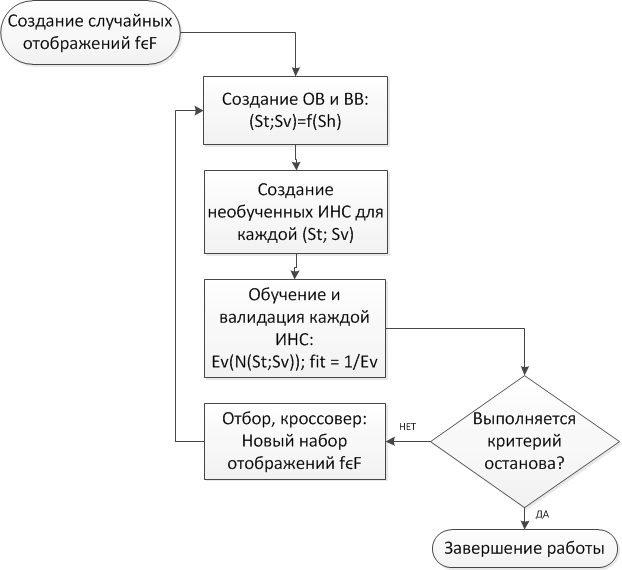
\includegraphics[width=0.4\textwidth]{algo.png}
  }
\end{figure}

При хранении экземпляр кодировался линейной последовательностью исполняемых команд и списком команд, результаты выполенения которых попадают в обучающую выборку. Такая структура данных не способствовала тонкой настройке алгоритмов кроссовера и мутации.

\section{Недостатки системы}
При работе со старой системой был выявлен быстрый рост размера экземпляров в ходе работы генетического алгоритма, в результате чего росло количество лишних данных и вычислений. Также в ней использовался крайне примитивный и плохонастраиваемый алгоритм мутации, предположительно не являющийся наилучшим. В прошлой версии системы использовалось распределеннные вычисления, что, хотя и позволяло использовать большие вычислительные мощности, неоправданно усложняло процесс эксплуации. 
\section{Постановка задачи учебно-исследовательской работы}
Основной задачей являлась разработка новой версии программного обеспечения для оптимизации обучающих выборок при помощи генетического алгоритма на основе старой с реализацией ряда модификаций:
\begin{enumerate}
\item Модификация формата вывода данных для облегчения взаимодействия с пользователем;
\item Устранение избыточности обучающих данных для снижения вычислительной мощности;
\item Модификация алгоритма мутации для реализации рекурсивной мутации.
\end{enumerate}

\chapter{Разработка и реализация модернизированной системы оптимизации обучающих выборок}
\section{Разработка системы оптимизации обучающих выборок}
\subsection{Модификация структуры вывода данных}
\par{\normalsize В силу тяжести взаимодействия пользователя с исходным форматом вывода данных было решено сменить этот формат. Целями смены формата были: повышение человекочитаемости, повышение легкости транспортировки и модифицирования данных эксперимента, по возможности сохранение легкости загрузки данных в приложение.
Возможными структурами хранения при решении данной задачи были XML, JSON, исполняемый код или база данных.}
\begin{longtable}{|p{0.16\linewidth}|p{0.26\linewidth}|p{0.26\linewidth}|p{0.26\linewidth}|}
\multicolumn{4}{l}{\tablename~\ref{T:Ta} ~Сравнение возможных структур хранения данных \label{T:Ta}}\\
\hline
Средство & Читаемость & Передача & Скорость \\
\hline
\endfirsthead
\multicolumn{4}{l}{Продолжение таблицы~\ref{T:Ta}}\\
\hline
Средство & Читаемость & Передача & Скорость \\
\hline
\endhead\small
XML & Читаемый в сыром виде формат. Для прочтения в удобном виде достаточно элементарного браузера. & Для передачи достаточно просто переслать интересующее поддерево или файл целиком. & Парcинг требует затрат времени. Затраты, однако, можно сократить оптимизацией, основанной на жесткости структуры.   \\ \hline
JSON & Читаемость формата в сыром виде несколько затруднена. Требуется специальный просмотровщик. & Для передачи достаточно переслать интересующий объект или файл целиком. & Парсинг требует минимального времени --- фактически это преобразование из строки в код. \\ \hline
Исполняемый код & Читаемость формата в сыром виде требует специальных навыков. Желательна подсветка синтаксиса и знание структуры программы. & Для передачи данных достаточно передать цельный кусок кода, что тоже требует специальных навыков. & Парсинг требует минимального времени --- фактически это преобразование из строки в исполняемый код. \\ \hline
База данных &
Читаемость в сыром почти невозможна. Требуются специальные просмотровщики. Цельность данных с точки зрения просмотра теряется. &
Передача данных как таковых требует либо объединенной БД для нескольких экземпляров системы, между которыми идет передача, либо выгрузки из базы данных. &
Скорость работы зависит от СУБД и скорости соединения, если база данных удалена, однако скорость работы любой базы данных на локальной машине --- выше, чем скорость преобразования текстовых файлов. \\ 
\hline
\end{longtable}
\normalsize
По результатам анализа разницы между представленными альтернативами был выбран формат данных XML. [\ref{XML}]

\subsection{Устранение избыточности обучающих данных}
В предыдущей версии возникла проблема избыточности размера экземпляров, которая достаточно критично влияла на объем  вычислений, производимых системой. Задачей является сокращение роста экземпляров при сохранении возможности такого роста.

Устранить избыточность обучающих данных можно было при помощи нескольких модификаций:
\begin{enumerate}
\item Отбрасывание на каждой мутационной фазе алгоритма одного элемента из экземпляра и проверка направления изменения фитнесс-функции;
\item Жесткое ограничение на размер экземпляра;
\item Изменение распределения вероятностей в пользу уменьшения, а не увеличения размера экземпляра.
\end{enumerate}
Вариант с жестким ограничением на размер экземпляра был отвергнут в связи с невозможностью в общем случае предугадать реальную правильную длину. Вариант с изменением алгоритма мутации был исключен в силу увеличения времени работы каждого шага почти в два раза. Реализуемым вариантом стал вариант с изменением распределения вероятностей. Конкретным изменением послужило увеличение возможного интервала размеров на следующем шаге в сторону уменьшения.

\subsection{Модификация алгоритма мутации для реализации рекурсивной мутации}
Для осуществления возможности вносить большее разнообразие в экземпляры и большей настраивамости хода работы алгоритма требовалось введение возможности мутировать не только атомарные объекты, но и объединяющие их структуры.

Для реализации рекурсивной мутации в каждой сущности (вплоть до атомарного элемента --- функции ЦОС) была модифицирована процедура мутации. На фазе мутации каждая сущность верхнего уровня с заданной вероятностью мутировала полностью --- генерировался новый экземпляр этой сущности, в обратном же случае она вызывала мутацию всех своих сущностей-детей.

\section{Реализация системы оптимизации обучающих выборок}
Текущая версия ПО представляет из себя пакет скриптов на языке python версии 2.7, содержащий инструменты для проведения вычислений и анализа результатов.

Алгоритм по существу не менялся по сравнению с прошлой версией. Однако изменению подверглись его подалгоритмы и методы реализации.

Модуль вычислений описан в диаграмме классов \ref{class-diagram}
\begin{figure}[H]
 \centering{
 	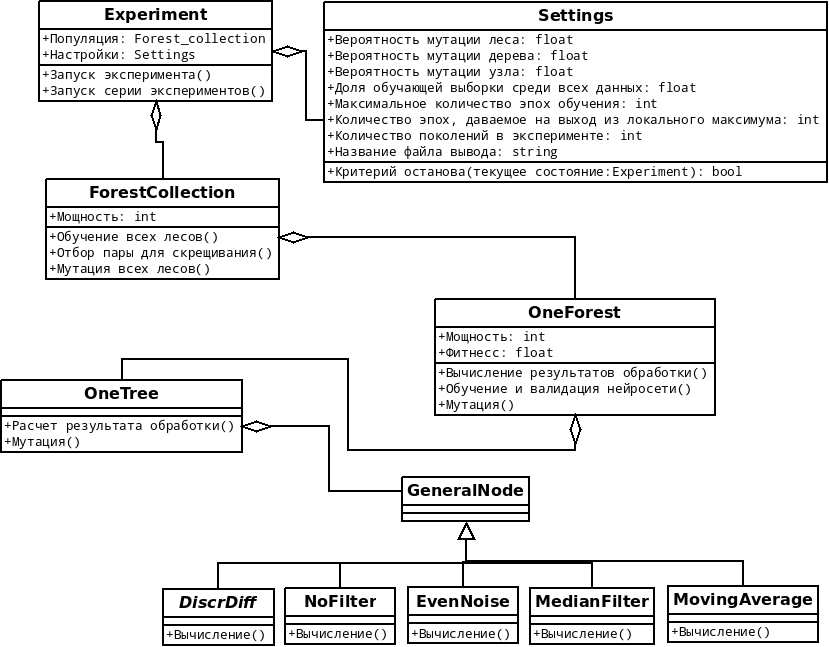
\includegraphics[width=0.9\textwidth]{class-diagram.png}
  }
  \caption{диаграмма классов модуля проведения вычислений}\label{class-diagram}
\end{figure}
Для инициализации вычислений требуется представить входные данные для обработки и входные данные для вычислительного модуля. Стандартным методом получения данных для обработки является набор csv-файлов со значениями. Входные данные для вычислительного модуля фактически представляют собой экземпляр класса настроек. Выходные данные вычислительного модуля представлены в XML-формате и выгружаются в файл с настраиваемым названием.

Модуль обработки результатов вычислений представляет собой набор скриптов, позволяющих собирать информацию о ходе и результатах генетического алгоритма как с одного, так и с набора XML-файлов. По результатам работы модуль строит csv-файл, содержащий в себе выбранные и обработанные значения.
 
\par{Используемые библиотеки:}
\par{PyBrain --- для создания и обучения искусственных нейросетей;}
\par{SciPy и NumPy --- для ускорения вычислений.} \cite{SciPy}

\chapter{Тестирование разработанной системы}
\section{Используемые тестовые сценарии}
Для тестирования использовалось два типа систем: линейная и нелинейная. Под сценарием эксперимента подразумевается набор из входных и целевых данных для нейросети. \cite{Neural_Networks}
\subsection{Линейная система}
Пусть существует бассейн, который является объектом управления. К нему подведены две трубы: через одну в бассейн может поступать вода с произвольной скоростью (в данном тестовом сценарии не будут учитываться физические ограничения), через вторую трубу вода может уходить из бассейна с произвольной скоростью. Через эти две трубы осуществляется управление бассейном. Ограничения на то, что объем воды в бассейне должен быть неотрицательным нет, но, стоит отметить, что в данном сценарии не возникает соответствующей ситуации.\\
Пусть существуют следующие экспериментальные данные:\\
$ X^{(0)} $ – объем поступившей за $ \Delta t $ воды;\\
$ X^{(1)} $ – объем откачанной за $ \Delta t $ воды;\\
$ X^{(2)} $ – объем воды, находящейся в бассейне в данный момент времени;\\
$ X^{(3)} $ – посторонний сигнал, отличающийся от остальных;\\
Бассейн реагирует на управляющие воздействия следующим образом:\\
\begin{equation}
X^{(2)}_{i} = X^{(2)}_{i-1} + X^{(0)}_{i-1} - X^{(1)}_{i-1}; X^{(2)}_{0}=10
\end{equation}


Пусть испытуемая система не имеет априорной информации об объекте управления и имеет доступ к следующим данным в качестве исходных:\\
$ X^{(0) \Delta t} $ – объем поступившей за $ \Delta t $ воды, на этот сигнал наложен импульсный шум (inflow\_noizd);\\
$ X^{(1) \Delta t} $ – объем откачанной за $ \Delta t $ воды (outflow);\\
$ X^{(3)} $ – посторонний сигнал (trash).\\
\subsection{Нелинейная система}
Пусть $ X^{(0)}, .., X^{(5)}$ --- действительные временные ряды из которых $ X^{(3)}, .., X^{(5)}$ не оказывают на систему никакого воздействия.\\
$ X^{(6)} $ --- выход системы.

Cистема реагирует на управляющие воздействия следующим образом:\\
\begin{equation}
X^{(6)}_{i} = |X^{(0)} - X^{(1)}| + X^{(2)}
\end{equation}
Перед подачей в вычислительный модуль на $ X^{(0)} $ был наложен постоянный шум с амплитудой 0.5, на $ X^{(1)} $ наложен шум, прибавляющий или вычитающий 1 с вероятностями по 2.5\% (условно такой шум можно считать импульсным). Остальные сигналы зашумлению не подвергались.

\section{Экспериментальная проверка работоспособности системы}
В прошлой версии для анализа хода работы системы использовался метод, предполагающий постановку одного эксперимента с большим размером популяции. Для аналогичных целей в данной работе был использован метод, предполагающий постановку серии экспериментов с малым размером популяции и усреднение данных среди нескольких экспериментов с одинаковыми условиями. Предполагалось, что данный метод позволит усматривать более тонкие зависимости за счет увеличения времени сходимости, а усреднение данных среди нескольких экспериментов позволит избежать влияния случайных совпадений среди сгенерированной стартовой популяции. \cite{SelfSystems}
\subsection{Работоспособность модуля для линейной системы}
Для проверки работоспособности модуля при прогнозировании работы линейной системы из серии экспериментов с использованием линейного тестового сценария был выбран лучший экземпляр и построен прогноз, данный нейронной сетью, обученной лучшим экземпляром, в сравнении с истинными значениями. Результаты построения приведены на рисунке \ref{linear_work}. Прогноз строился для контрольной части данных.
\begin{figure}[H]
 
 \centering{
 	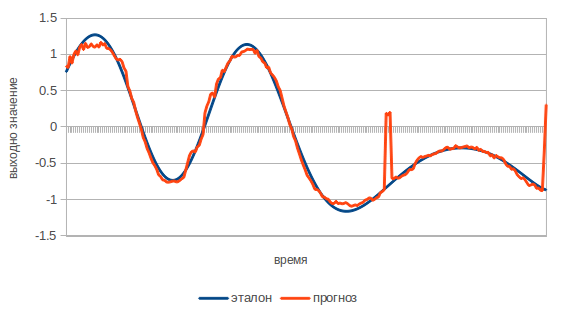
\includegraphics[width=0.65\textwidth]{linear_work.png}
  }
  \caption{Результаты прогноза и эталонная функция выхода}\label{linear_work}
\end{figure}
Доверительный интервал с уровнем доверия 98\% оказался равен $ \pm 0.3 $
\subsection{Работоспособность модуля для нелинейной системы}
Для проверки работоспособности модуля при прогнозировании работы нелинейной системы из серии экспериментов с использованием нелинейного тестового сценария был выбран лучший экземпляр и построен прогноз, данный нейросетью, обученной лучшим экземпляром, в сравнении с истинными значениями. Результаты построения приведены на рисунке \ref{nonlinear_work}. Прогноз строился для контрольной части данных.
\begin{figure}[H]
 
 \centering{
 	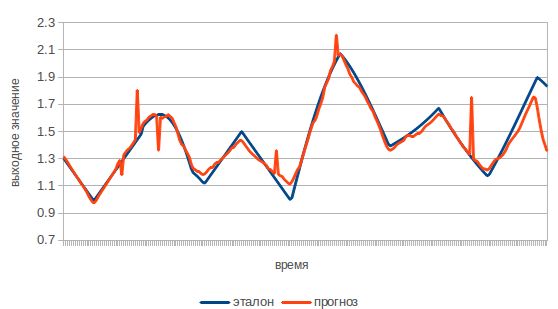
\includegraphics[width=0.65\textwidth]{nonlinear_work.png}
  }
  \caption{Результаты прогноза и эталонная функция выхода}\label{nonlinear_work}
\end{figure}
Доверительный интервал с уровнем доверия 97\% оказался равен $ \pm 0.3 $
\subsection{Устранение избыточности}
В качестве эксперимента для проверки работоспособности решения по устранению избыточности было решено провести пару тестов на одинаковых входных данных для старого и нового алгоритмов кроссовера. В качестве метрики для сравнения был выбран размер экземпляра на определенной итерации, усредненный среди нескольких экспериментов, для устранения возможности влияния случайных факторов.
\begin{figure}[H]

 \centering{
 	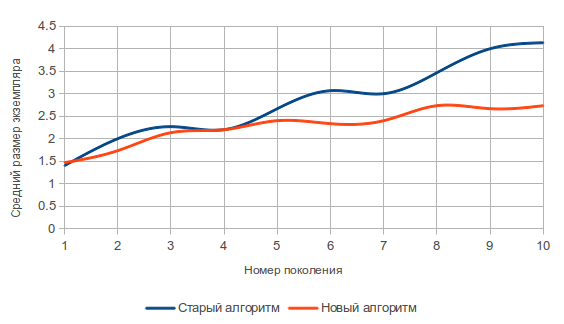
\includegraphics[width=0.6\textwidth]{crossover_difference.png}
  }
   \caption{Средние размеры экземпляров по поколениям для старого и нового алгоритма}\label{cross_diff}
\end{figure}
Средняя производная по таким графикам различается в два раза в пользу новой версии алгоритма кроссовера, что говорит о существенном снижении объемов избыточных данных в обучающей выборке. Важно также отметить, что истинным размером является два, что близко к полученному в этом эксперименте для нового алгоритма. 

\subsection{Модернизация алгоритма мутации}
Для оценки качества модификации алгоритма мутации было проведено равное количество экспериментов при одинаковых начальных условиях для старого и нового алгоритма мутации для разных вероятностей мутации. Для моделирования старого алгоритма (плоский случай) новому задавались нулевыми вероятности мутации всех элементов кроме атомарных --- функций ЦОС. Для моделирования алгоритма с использованием рекурсивной мутации вероятности выставлялись одинаковыми и равными приведенной вероятности рассчитаной по формуле \ref{equiv_prob}
\begin{equation}
P_{n}=\sqrt[3]{p-1}+1
\label{equiv_prob}
\end{equation}
, где $ p $ --- вероятность для плоского случая (приведенная вероятность), а $ P_{n} $ --- аналогичная ей вероятность для рекурсивного случая.

На основе экспериментов, проведенных с линейной системой, построены графики, приведенные на рисунках \ref{mutate_diff_fit} и \ref{mutate_diff_gen}. На основе графика  \ref{mutate_diff_gen} можно сказать, что после реализации новой версии мутации уменьшилось время сходимости алгоритма, а также на графике \ref{mutate_diff_fit} видно, что фитнесс-функция оптимального экземпляра не только не ухудшилась, но и улучшилась при таком переходе.
\begin{figure}[H]
 
 \centering{
 	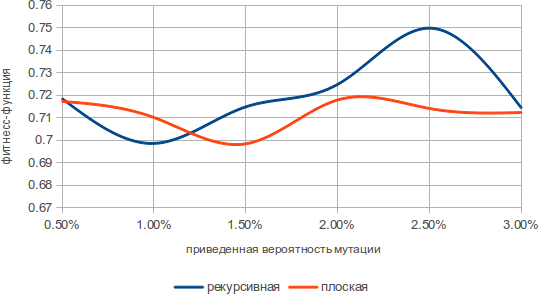
\includegraphics[width=0.6\textwidth]{mutation_difference_fit.png}
  }
  \caption{средняя фитнесс-функция для приведенных вероятностей мутации}\label{mutate_diff_fit}
\end{figure}
\begin{figure}[H]
 
 \centering{
 	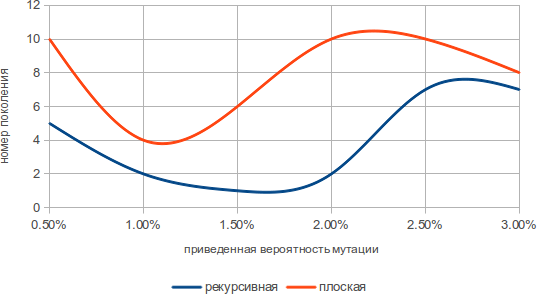
\includegraphics[width=0.6\textwidth]{mutation_difference_gen.png}
  }
  \caption{время сходимости для приведенных вероятностей мутации}\label{mutate_diff_gen}
\end{figure}


На основе экспериментов, проведенных с нелинейной системой, построены графики, приведенные на рисунках \ref{mutate_diff_fit_nl} и \ref{mutate_diff_gen_nl}. Средние и максимальные значения на графике \ref{mutate_diff_fit_nl} для рекурсивной и плоской мутации оказались примерно равными. То есть в пределах поставленных экспериментов нельзя сказать, что какая-либо из представленных функций сходится к более высокому значению. Как видно на графике \ref{mutate_diff_gen_nl}, рекурсивный алгоритм почти всегда сходится быстрее, а также сходится быстрее в среднем.
\begin{figure}[H]
 
 \centering{
 	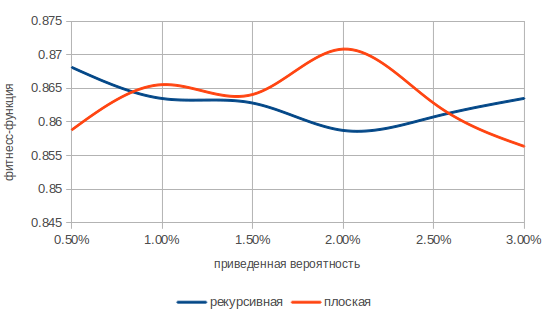
\includegraphics[width=0.625\textwidth]{mutation_difference_fit_nl.png}
  }
  \caption{средняя фитнесс-функция для приведенных вероятностей мутации}\label{mutate_diff_fit_nl}
\end{figure}
\begin{figure}[H]
 
 \centering{
 	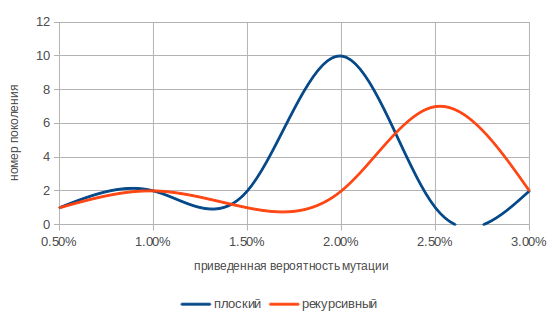
\includegraphics[width=0.625\textwidth]{mutation_difference_gen_nl.png}
  }
  \caption{время сходимости для приведенных вероятностей мутации}\label{mutate_diff_gen_nl}
\end{figure}


\subsection{Модификация структуры вывода данных}
В силу вычислительной сложности задачи эксперименты зачастую ставились на сторонней машине, после чего результаты вычислений пересылались для анализа на основную машину. Путь передачи с копированием XML-файлов показал себя как надежный и простой. За время передачи данных не произошло ни одной потери и синхронная включенность обеих машин не требовалась для передачи данных.
\section{Результаты анализа экспериментов}
В ходе тестирования разработанной системы были получены следующие результаты:
\begin{enumerate}
\item Разработанная система способна найти субоптимальное решение как для линейной, так и для нелинейной системы. Обученная нейросеть в таком случае дает прогноз для доверительного интервала $ \pm 0.3 $ в 98\% и 97\% соответственно;
\item Модификация алгоритма для устранения избыточности позволяет снизить прирост размера экземпляров в два раза;
\item Модернизация алгоритма мутации способна ускорить сходимость и, по крайней мере в некоторых случаях, улучшить результаты поиска;
\item Был использован новый метод исследования работы алгоритма, который, однако, при увеличении сложности анализа и вычислительной сложности не дал положительного прироста информативности.
\end{enumerate}

% endof %

\backmatter %% Здесь заканчивается нумерованная часть документа и начинаютяс заключение и ссылки

\Conclusion % заключение к отчёту

В результате данной работы была разработана и реализована новая версия программного обеспечения для оптимизации обучающих выборок с помощью генетического алгоритма. В ходе разработки были проведены модификации алгоритмов некоторых модулей системы, позволившие достигнуть улучшения работы системы по сравнению с предыдущей версией. В процессе реализации был использован набор сторонних библиотек, что позволило упростить дальнейшее модифицирование системы и уменьшить объем реализуемого исходного кода (PyBrain для работы с нейронными сетями и SciPy + NumPy для вычислительных задач). Был проведен переход системы на другой язык программирования (Python 2.7) и использование системы контроля версий (git) для упрощения дальнейшей модификации и поддержания системы.

В результате тестирования разработанной системы были получены следующие новые результаты:
\begin{enumerate}
\item Система показала работоспособность в случае нелинейных систем. То есть способность найти субоптимальное решение такое, что прогноз укладывается в доверительный интервал $ \pm 0.3 $ с вероятностью 97\% для исследованной системы;
\item Модификация алгоритма для устранения избыточности позволяет снизить прирост размера экземпляров в два раза;
\item Модернизация алгоритма мутации способна ускорить сходимость и, по крайней мере в некоторых случаях, улучшить результаты поиска.
\end{enumerate}


\begin{thebibliography}{1} %% здесь библиографический список

\bibitem{HSWGCroatia}
{Oreski} S., {Oreski} D., {Oreski} G.
\newblock Hybrid system with genetic algorithm and artificial neural networks and its
application to retail credit risk assessment.
\newblock // Expert Systems with Applications. 2012 \No \ 39 С. 12605–12617

\bibitem{Clever_Algorithms}
{Brownlee} J.
\newblock Clever Algorithms: Nature-Inspired Programming Recipes.
\newblock ISBN: 978-1-4467-8506-5, 2012. 438 c.

\bibitem{Neural_Networks}
{Комашинский} В.И., {Смирнов} Д.А.
\newblock К63 Нейронные сети и их применение в системах управления и связи.
\newblock М.: Горячая линия-Телеком, 2003. 94 c. ISBN 5-93517-094-9

\bibitem{AI}
{Жданов} А.А.
\newblock Автономный искусственный интеллект 2-е изд.
\newblock М.: БИНОМ. Лаборатория знаний, 2009. 359 c. ISBN 978-5-94774-995-3

\bibitem{SelfSystems}
{Николенко} С.И., {Тулупьев} А.Л.
\newblock Н63 Самообучающиеся системы.
\newblock М.: МЦНМО, 2009. 288 c. ISBN 978-5-940570-506-1

\bibitem{DataMining}
{Han} J., {Kamber} M., {Pei} J.
\newblock Data mining: concepts and techniques 3-rd ed.
\newblock ISBN 978-0-12-381479-1

\bibitem{GAinClassifier}
{Gabrys} B., {Ruta} D.
\newblock Genetic algorithms in classifier fusion
\newblock // Applied Soft Computing. 2006 \No \ 6 С. 337-347

\bibitem{SciPy}
{Oliphant} T.E.
\newblock Python for Scientific Computing
\newblock // Computing in Science \& Engineering. 2007 \No \ 9 С. 10-20

\end{thebibliography}

\newpage
\appendix
\chapter{Пример экземпляра популяции генетического алгоритма записанного в XML}
\label{XML}
\begin{lstlisting}

<forest power="4"  fitness="0.839943138225">
<tree input="xor2" power="5">
<node function="MedianFilter" enter_params="{'frame': 3}"/>
<node function="DiscrDiff" enter_params="{}"/>
<node function="MedianFilter" enter_params="{'frame': 5}"/>
<node function="EvenNoise" enter_params="{'frame': 0}"/>
<node function="MedianFilter" enter_params="{'frame': 7}"/>
</tree>
<tree input="trash3" power="2">
<node function="DiscrDiff" enter_params="{}"/>
<node function="NoFilter" enter_params="{}"/>
</tree>
<tree input="trash1" power="3">
<node function="MedianFilter" enter_params="{'frame': 7}"/>
<node function="NoFilter" enter_params="{}"/>
<node function="DiscrDiff" enter_params="{}"/>
</tree>
<tree input="trash3" power="5">
<node function="DiscrDiff" enter_params="{}"/>
<node function="EvenNoise" enter_params="{'frame': 0}"/>
<node function="MedianFilter" enter_params="{'frame': 7}"/>
<node function="EvenNoise" enter_params="{'frame': 0}"/>
<node function="MovingAverage" enter_params="{'window': 7}"/>
</tree>
</forest>
\end{lstlisting}

% \bibliography{biblio/filosofy} %% вместо вставки библиографии можно использовать базы BiBTeX - просто раскомментируйте эту строку.
\end{document}
